\section{SNR on Monolingual Models}
\label{app:snr-monolingual}

No surrogate we test predicts decision accuracy well on our ladder (\S\ref{sec:rq3}), while \citet{heineman_signal_2025} find that SNR does on English models. We test whether the difference comes from the multilingual setting or from our implementation. We compute the SNR--DA relation with the same code on three populations: the English DataDecide ladder of \citet{heineman_signal_2025}, our English-only models ($K=1$), and our multilingual models, all read on the same English benchmarks.

\textbf{Setup.} The benchmarks are the nine tasks of the OLMES suite used by \citet{heineman_signal_2025} that we also evaluate: ARC-Easy, ARC-Challenge, BoolQ, CommonsenseQA, HellaSwag, MMLU, OpenBookQA, PIQA and WinoGrande. CommonsenseQA and MMLU are read in their answer-text (RF) version, which matches the cloze format of DataDecide. SNR is the relative-standard-deviation SNR of Appendix~\ref{app:surrogates}: the spread of the final scores across the models of a size, divided by the checkpoint noise. DA-size is the multi-axis DA of each proxy against the reference.
\begin{itemize}[leftmargin=*,itemsep=0pt,topsep=2pt]
    \item \textbf{DataDecide}: the 25 data recipes at 150M, 300M and 750M against the 1B reference, recomputed from the released evaluations with our code.
    \item \textbf{Ours}: four model configurations per language setting, the proxies 90M--1B against 1.7B, seed 1904, with the above-chance threshold applied. At $K=1$ the four are the deep models on DCLM-Edu, on DCLM without the educational filter and on FineWeb, and the shallow model on DCLM-Edu. At $K=2$, 15 and 30 they are the mirrored configurations: the base and shallow models, with the Spanish and Chinese swaps at $K=2$ and the scheme-B and $T=3$ builds at $K=15$ and 30. Four configurations give six pairs per decision.
\end{itemize}
For each population, we compute Spearman's $\rho$ between log SNR and DA-size over its (benchmark, proxy size) points, with a 95\% bootstrap interval that resamples whole benchmarks.

\begin{figure*}[t]
\centering
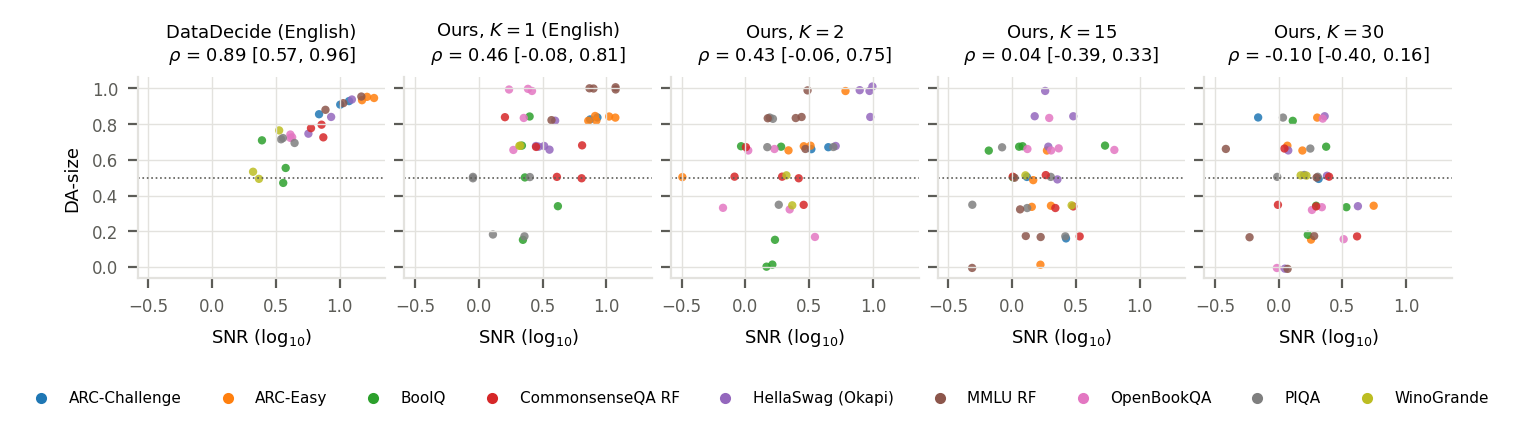
\includegraphics[width=\textwidth]{figures/app_snr_monolingual.png}
% source: src/signal-and-noise/analysis/rq13_english_only/pretraining/predictivity/english_only_allenai_snr_da_paper.png (allenai_snr.py)
\caption{\textbf{SNR predicts decision accuracy on English models and stops doing so as the models become multilingual.} Each point is one benchmark at one proxy size: its log SNR against its DA-size, on the nine OLMES benchmarks. The first panel is DataDecide (25 data recipes, 150M--750M against 1B); the others are our models at each number of languages $K$ (four configurations, 90M--1B against 1.7B). The title gives Spearman's $\rho$ with its 95\% bootstrap interval over benchmarks. The dotted line is chance agreement.}
\label{fig:app_snr_monolingual}
\end{figure*}

\begin{table*}[t]
\centering
\small
\begin{adjustbox}{max width=\textwidth}
\begin{tabular}{lrrrrrrrrrr}
\toprule
 & \multicolumn{2}{c}{DataDecide} & \multicolumn{2}{c}{L1} & \multicolumn{2}{c}{L2} & \multicolumn{2}{c}{L15} & \multicolumn{2}{c}{L30} \\
\cmidrule(lr){2-3}\cmidrule(lr){4-5}\cmidrule(lr){6-7}\cmidrule(lr){8-9}\cmidrule(lr){10-11}
Benchmark & SNR & DA & SNR & DA & SNR & DA & SNR & DA & SNR & DA \\
\midrule
ARC-Challenge & 10.1 & 0.90 & 8.0 & 0.83 & 3.9 & 0.67 & 2.0 & 0.33 & 1.4 & 0.67 \\
ARC-Easy & 16.4 & 0.95 & 8.4 & 0.83 & 2.9 & 0.67 & 1.7 & 0.33 & 1.8 & 0.67 \\
BoolQ & 3.6 & 0.56 & 2.3 & 0.50 & 1.6 & 0.17 & 1.1 & 0.67 & 2.0 & 0.33 \\
CommonsenseQA RF & 7.2 & 0.77 & 4.1 & 0.67 & 1.9 & 0.50 & 2.2 & 0.33 & 2.0 & 0.33 \\
HellaSwag (Okapi) & 8.6 & 0.83 & 3.3 & 0.67 & 9.4 & 1.00 & 1.9 & 0.83 & 2.3 & 0.50 \\
MMLU RF & 10.7 & 0.91 & 7.9 & 1.00 & 2.8 & 0.83 & 1.2 & 0.17 & 1.2 & 0.17 \\
OpenBookQA & 4.1 & 0.71 & 2.3 & 1.00 & 1.7 & 0.33 & 2.0 & 0.67 & 2.2 & 0.33 \\
PIQA & 3.6 & 0.71 & 1.3 & 0.50 & 1.6 & 0.67 & 1.3 & 0.33 & 1.6 & 0.50 \\
WinoGrande & 2.3 & 0.54 & 2.1 & 0.67 & 2.2 & 0.42 & 2.1 & 0.42 & 1.6 & 0.50 \\
\midrule
Median & 6.0 & 0.76 & 2.9 & 0.67 & 2.2 & 0.67 & 1.7 & 0.50 & 1.8 & 0.50 \\
$\rho$(log SNR, DA) & \multicolumn{2}{c}{0.89} & \multicolumn{2}{c}{0.46} & \multicolumn{2}{c}{0.43} & \multicolumn{2}{c}{0.04} & \multicolumn{2}{c}{-0.10} \\
\bottomrule
\end{tabular}

\end{adjustbox}
% source: src/signal-and-noise/analysis/rq13_english_only/pretraining/predictivity/english_only_allenai_snr_da.tex (allenai_snr.py)
\caption{\textbf{SNR and DA-size of the OLMES benchmarks on English and multilingual models.} Per benchmark, the median over the proxy sizes of the SNR and of DA-size, for DataDecide and for our models at each $K$, and Spearman's $\rho$ between log SNR and DA-size over all (benchmark, proxy) points. On our side, DA-size moves in steps of 1/6 (six pairs).}
\label{tab:app_snr_monolingual}
\end{table*}

\textbf{Findings.}
\begin{itemize}[leftmargin=*,itemsep=2pt,topsep=2pt]
    \item \textbf{Our code reproduces the English result.} On DataDecide, log SNR and DA-size correlate at $\rho = 0.89$ (95\% interval 0.57--0.96), in line with the strong relation reported by \citet{heineman_signal_2025} (Figure~\ref{fig:app_snr_monolingual}).
    \item \textbf{On our English-only models, SNR still tracks DA.} At $K=1$, $\rho = 0.46$, and at $K=2$, where English is joined by one language, $\rho = 0.43$. As on DataDecide, the ARC tasks and MMLU have the highest SNR (7.9--8.4) and a high DA-size (0.83--1.00). With nine benchmarks and six pairs per decision, both intervals include zero ($-0.08$ to 0.81 and $-0.06$ to 0.75).
    \item \textbf{With many languages, the relation disappears.} On the same English benchmarks, $\rho = 0.04$ at $K=15$ and $-0.10$ at $K=30$. The median SNR falls from 6.0 on DataDecide and 2.9 at $K=1$ to 1.7--1.8 at $K=15$ and 30, and the median DA-size from 0.67 at $K=1$ and 2 to 0.50 (Table~\ref{tab:app_snr_monolingual}). ARC-Easy, for example, has an SNR of 16.4 on DataDecide, 8.4 at $K=1$ and 1.7--1.8 at $K=15$ and 30.
\end{itemize}

The decisions differ across the populations: DataDecide compares data recipes, our $K=1$ models compare English corpora and depth, and our multilingual models compare language lists and depth. DataDecide also reads the checkpoint noise over its last five saved checkpoints. The levels are therefore not directly comparable. The direction is consistent, however: the same code finds the SNR--DA relation on English models and loses it on the same English benchmarks as the number of training languages grows. This supports reading the weak surrogates of \S\ref{sec:rq3} as a property of multilingual training rather than of our implementation.
